\begin{refsection}[research/ishikawa/group.bib]
\nocite{*}
\chapter{System Software Research Team}
%=============================================================================
\section{Members}
%=============================================================================

\begin{itemize}
  \item[] Yutaka Ishikawa (Team Leader)
  \item[] Atsushi Hori (Senior Scientist)
  \item[] Yuichi Tsujita (Research Scientist)
  \item[] Kazumi Yoshinaga (Postdoctoral Researcher)
  \item[] Akio Shimada (Research Associate)
  \item[] Masayuki Hatanaka (Research Associate)
  \item[] Norio Yamaguchi (Research Associate)
  \item[] Toyohisa Kameyama (Technical Staff)
\end{itemize}

%=============================================================================
\section{Research Activities}
%=============================================================================
The system software team focuses on the research and development of an
advanced system software stack not only for the "K" computer but also
for towards exascale computing.  There are several issues in carrying
out future computing. Two research categories are taken into account:
i) scalable high performance libraries/middleware, such as file I/O
and low-latency communication, and ii) a scalable cache-aware, and
fault-aware operating system for next-generation supercomputers based
on many core architectures.

%==============================================================================
\section{Research Results and Achievements}
%==============================================================================

%------------------------------------------------------------------------------
\subsection{PRDMA (Persistent Remote Direct Memory Access)}
%------------------------------------------------------------------------------
%The goal of this research is to design and evaluate an efficient MPI
%implementation for neighborhood communication by taking advantage of
%the Tofu interconnect, which has multiple RDMA (Remote Direct Memory
%Access) engines and network links per MPI process. The neighborhood
%communication pattern is commonly used in the ghost (or halo) cell
%exchanges.

The PRDMA (Persistent RDMA)\cite{dist-prdma} is an enhancement of MPI persistent
communication primitives to reduce the communication latency and to
improve the overlap between computation and communication over an
RDMA-enabled interconnect. The RDMA-base transfers can progress the
non-blocking communication without CPU intervention, and reduce extra
copy overheads and memory consumption for data transfers due to the
Zero-Copy feature. The MPI persistent communication is defined in MPI
standard since MPI version 1.1 specification. For example, when
calling with the same communication parameters from an iterative
stencil loop, the MPI persistent communication can avoid the redundant
setup cost on every call, including the RDMA buffer address
exchanges. Also, the initial costs to schedule the communication
requests are amortized over a number of stencil iterations.

We implemented the prototype of the PRDMA protocol over the Open MPI
provided on the K computer in FY2012. In FY2013, We improved the
performance in the ghost cell exchange pattern, such as derived
datatype handling and special handling upon non-periodic boundary
condition.
Furthermore, we applied the PRDMA to an optimized prototype
implementation of MPI-3 Neighborhood Collectives, as known as
MPI\_Neighbor\_alltoallw, over MPICH on the K computer in FY2014.

In FY2015, we improved the quality of the MPICH on K computer, and
made it available for public use on the K computer. In addition, we
have been implementing the prototype of the PRDMA-based MPI-RMA
implementation on the Tofu2 interconnect of FX100 to compare with the
MPI-3 neighborhood collectives. The MPI-RMA passive synchronization
such as MPI\_Win\_lock / unlock does not require the involvement of
target process. To implement a truly passive locking on the FX100, we
designed a distributed lock queue using RDMA Atomic operations of
Tofu2 interconnect. In Figure \localref{fig:prdma}, the vertical axis shows the elapsed
time in second for 1000 calls of MPI\_Win\_lock and MPI\_Win\_unlock with
MPI\_LOCK\_SHARED, and the horizontal axis shows the number of MPI
processes which acquires the same lock. The FX10 indicates the result
of the Open MPI based generic implementation without RDMA Atomics. The
FX100 indicates the result of the MCS-based Readers-Writer lock
(Readers Preference) implementation using Tofu2 RDMA Atomics. The
FX100 achieves 130 [us] at 256 processes (114 [s] in FX10).

\begin{figure}
\begin{center}
 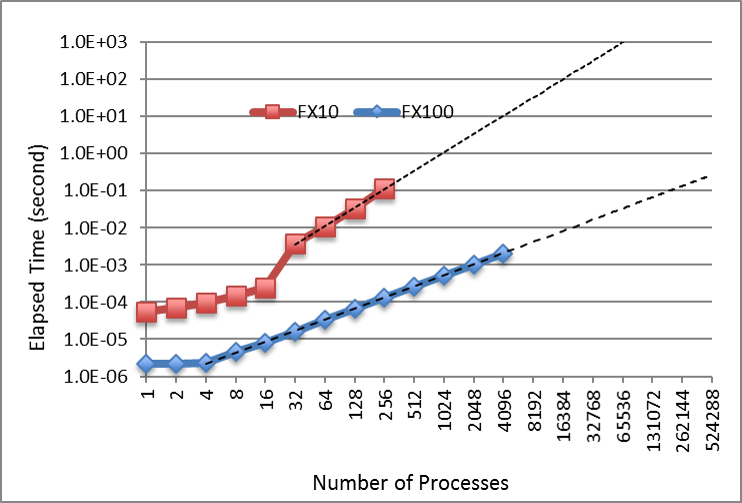
\includegraphics[width=0.7\textwidth,natwidth=557,natheight=377]{research/ishikawa/mpich-winlock.png}
\end{center}
  \caption{Benchmark Result of MPI\_Win\_lock / unlock with empty critical section}
  \locallabel{fig:prdma}
\end{figure}

%------------------------------------------------------------------------------
\subsection{OFI/LLC and RMPI}
%------------------------------------------------------------------------------
\begin{figure}
\begin{center}
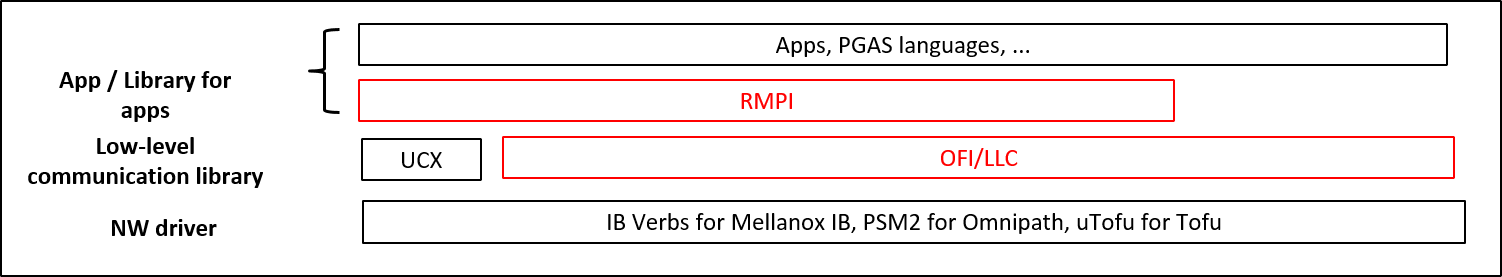
\includegraphics[width=0.8\textwidth,natwidth=1127,natheight=208]{research/ishikawa/mpich1.png}
\end{center}
 \caption{Relationships between applications, communication libraries and network driver}
 \locallabel{fig:mpich1}
\end{figure}

Two communication libraries have been developed. The first one is
called Low-Level Communication Library, which will adopt Open Fabric
Interface (OFI) and is called OFI/LLC. The second one is called
RIKEN-MPI (RMPI) which is based on MPICH. The relationships between
applications, RMPI, OFI/LLC and network drivers are explained by using
Figure \localref{fig:mpich1}. A network driver provides communication
functions to OFI/LLC. OFI/LLC provides communication functions to both
parallel language runtimes (e.g. MPI library) and applications
(e.g. visualization) via a low-level interface. RMPI provides
communication functions to applications via a high-level interface.

\begin{figure}
\begin{center}
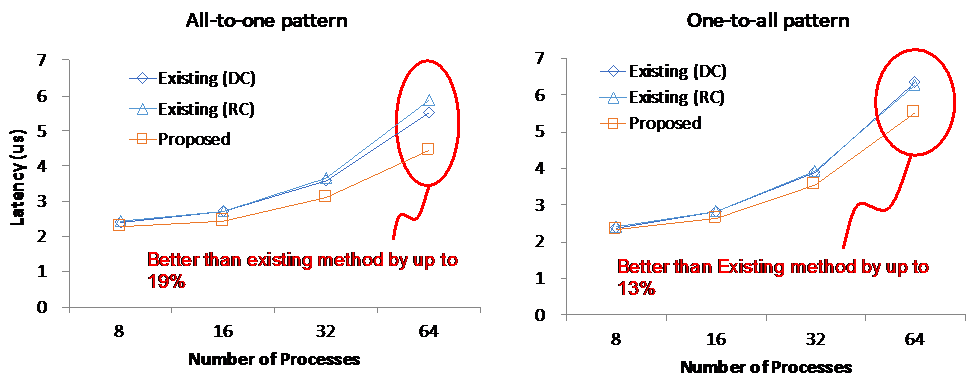
\includegraphics[scale=0.8,natwidth=703,natheight=276]{research/ishikawa/mpich2.png}
\end{center}
 \caption{Communication latency in all-to-one and one-to-all communication patterns}
 \locallabel{fig:mpich2}
\end{figure}

Two optimizations are performed in FY2015\cite{takagi2015}.  The first optimization
finds the proper numbers for different kinds of hardware contexts at
run-time.  The purpose is to maximize the performance while limiting
its memory consumption to the amount at which it is possible to run
parallel applications with millions of compute nodes.

The conventional network hardware provides a communication model in
which the memory-area for communication information for an end-point
pair (called context) is never released at run-time. The next
generation network hardware adds a new communication model in which
the memory-area can be allocated and released at run-time to save
memory. However, you lose performance just to make all end-point pairs
use the new model because it has a certain amount of performance
overhead when allocating. Therefore, it is needed to find how many
end-point pairs should use the conventional model and how many the new
model. We propose a method to find the proper combination of the
number-pair at run-time. This is done by calculating the benefits of
different combinations of the number-pair at run-time by using the
communication statistics and an analytic model. It was implemented
in OFI/LLC and evaluated using two micro-benchmarks performing
all-to-one and one-to-all types of communications. The latency is
reduced by up to 19\% and 13\%, respectively, as shown in Figure
\localref{fig:mpich2}.

\begin{table}
 \caption{Memory consumption per compute node of MPICH and LLC}
         \locallabel{tab:mpich}
%% 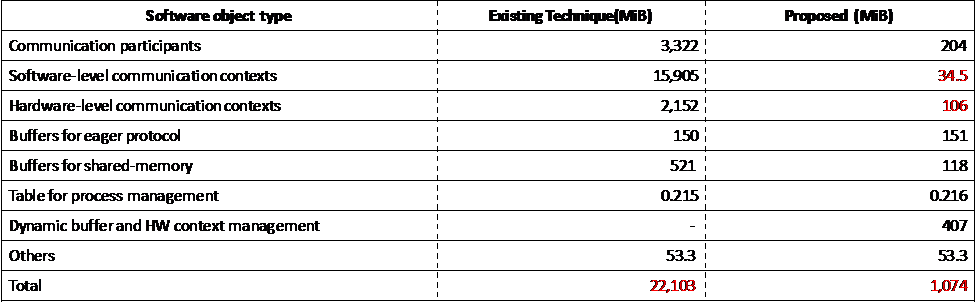
\includegraphics[natwidth=702,natheight=220]{research/ishikawa/mpich3.png}
\begin{center}
\begin{tabular}{l|r|r} \hline
Software object type &           Existing Technique (MiB) &      Proposed (MiB) \\ \hline
Communication participants &            3,322   & 204 \\
Software-level communication contexts & 15,905  & 34.5 \\
Hardware-level communication contexts & 2,152   & 106 \\
Buffers for eager protocol &            150     & 151 \\
Buffers for shared-memory &             521     & 118 \\
Table for process management &          0.215   & 0.216 \\
Dynamic buffer and HW context management & -    & 407 \\
Others &                                53.3    & 53.3 \\
Total &                                 22,103  & 1,074 \\ \hline
\end{tabular}
\end{center}
\end{table}

The second optimization is for the both OFI/LLC and RMPI libraries. It
tries to keep only active software contexts in memory. The
purpose is to limit the per-node memory consumption with the same
target as the first optimization.

The conventional communication libraries prepare software contexts of
the number proportional to the number of MPI processes. The proposed
method only keeps a constant number of software contexts in memory by
releasing inactive contexts when necessary. The mechanism was
evaluated by using an analytic model of the memory consumption which
is created by analyzing source code of OFI/LLC and MPICH. Table
\localref{tab:mpich} shows the memory consumption with 4,194,304 MPI
processes on 1,048,576 compute nodes. The proposed method reduces the
memory consumption per compute node from 22~GiB to 1~GiB when compared
to the existing technique.

%------------------------------------------------------------------------------
\subsection{Scalable MPI-IO Using Affinity-Aware Aggregation}
%------------------------------------------------------------------------------
\begin{figure}
\begin{center}
 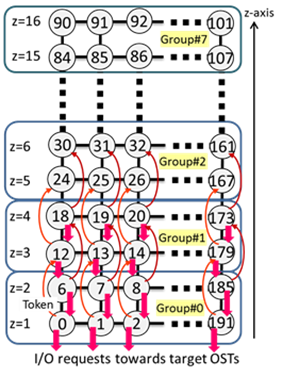
\includegraphics[width=0.5\textwidth,natwidth=204,natheight=271]{research/ishikawa/earth1.png}\\
(a) I/O throttling approach
\end{center}
\begin{center}
 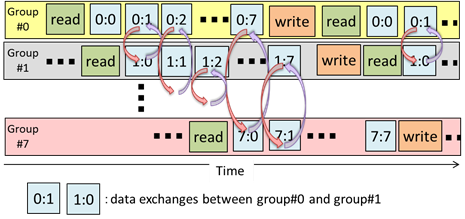
\includegraphics[width=0.7\textwidth,natwidth=335,natheight=158]{research/ishikawa/earth2.png}\\
(b) associated stepwise data exchanges
\end{center}
  \caption{Optimization Techniques in EARTH} \locallabel{fig:earth1}
\end{figure}

A commonly used MPI-IO library named ROMIO has the two-phase I/O
(TP-IO) scheme to improve collective I/O performance for
non-contiguous accesses. This research is addressing to optimize TP-IO
implementation for further I/O performance improvements than the
original one.
In the FY2015, we have proposed enhanced TP-IO approach named EARTH
(Effective Aggregation Rounds with THrottling) in the MPI library at
the K computer\cite{tsujita2015}. It has been arranged to have cooperative stepwise data
exchanges based on the optimized aggregator layout and I/O throttling
approach done in the FY2014. Its I/O throttling scheme and stepwise
data exchanges are illustrated in Figure \localref{fig:earth1}.

Figure \localref{fig:earth1}(a) illustrates I/O throttling approach of the
EARTH using token-relay. EARTH divided processes into groups which are
associated with target Object Storage Target (OST) of the FEFS file
system on the K computer. Then the EARTH throttles I/O request
generation of each process, where process that receives a token issues
I/O request. As a result, network and I/O request contention can be
minimized. Furthermore, stepwise data exchanges in Figure
\localref{fig:earth1}(b) improve data exchange times by splitting
all-to-all manner data exchanges into sub-groups which are associated
with I/O throttling. This stepwise data exchange scheme has two
advantages compared with the original all-to-all manner data
exchanges. One is minimization in waiting time to complete data
exchanges. Another is mitigation of network contention.

Performance evaluation was carried out using computing nodes ranged
from 192 to 3,072 nodes. I/O performance evaluation was done by using
the HPIO benchmark with non-contiguous access patterns on a local file
system of the FEFS on the K computer. The number of nodes was arranged
not to have any interference from other users' applications. In the K
computer case, we specified the number of nodes in a 3D manner node
allocation, where we chose the following five patterns; 2x3x32,
4x3x32, 8x3x32, 8x6x32, and 8x12x32. We deployed one MPI process per
one computing node, thus the number of MPI processes was the same with
that of used computing nodes. Figure \localref{fig:earth2} shows I/O
throughput values relative to the number of MPI processes.

\begin{figure}
\begin{center}
 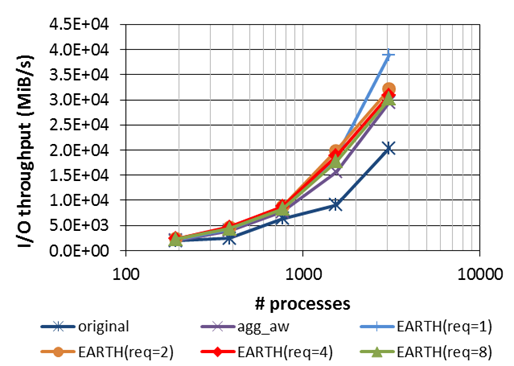
\includegraphics[natwidth=370,natheight=264]{research/ishikawa/earth3.png}
\end{center}
  \caption{I/O throughput of collective write}
  \locallabel{fig:earth2}
\end{figure}

In this evaluation, we examined the number of I/O requests for 1, 2,
4, and 8 in the I/O throttling scheme indicated by
{\it EARTH(req=1)}, {\it EARTH(req=2)}, {\it EARTH(req=4)},
and {\it EARTH(req=8)}, respectively
in addition to the original implementation indicated by {\it original}
and aggregator layout optimization only version ({\it agg\_aw}). The
EARTH optimization outperformed the original one and aggregator layout
optimization only version. From this evaluation, one I/O request case in
the EARTH optimization was the best when we had 3,072 processes. Our
future work is the way for tuning the number of I/O requests to gain
the best I/O performance.

%------------------------------------------------------------------------------
%\subsection{Partitioned Virtual Address Space}
\subsection{New Process / Thread Model}
%------------------------------------------------------------------------------
From FY2012, we have been developing a new process/thread model that
is suitable for the many-core architectures. The many-core
architectures are gathering attention towards the next generation
supercomputing. Many-core architectures have a large number of low
performance cores, and then the number of parallel processes within a
single node becomes larger on many-core environments. Therefore, the
performance of inter-process communication between the parallel
processes within the same node can be an important issue for parallel
applications.

Partitioned Virtual Address Space (PVAS) is a new execution model to
achieve high-performance inter-process communication on the many-core
environments. With PVAS, multiple processes run in the same virtual
address space as shown in Figure \localref{fig:pvas} to eliminate the
communication overhead due to the process boundaries that the current
modern OSes introduce for inter-process protection. In PVAS, the data
owned by the other process can be accessed by the normal load and
store machine instructions, just like the same way accessing the data
owned by itself. Thus, high-performance inter-process communication is
achieved.

We implemented the prototype of the PVAS execution model in the Linux
kernel in FY2012. We improved its quality and published it as open
source software in FY2013. To demonstrate the potential of PVAS, Open
MPI has been modified to utilize PVAS since then\cite{shimada2015}. Especially in
FY2015, proposed and developed PVAS was ported to McKernel.

\begin{figure}
\begin{center}
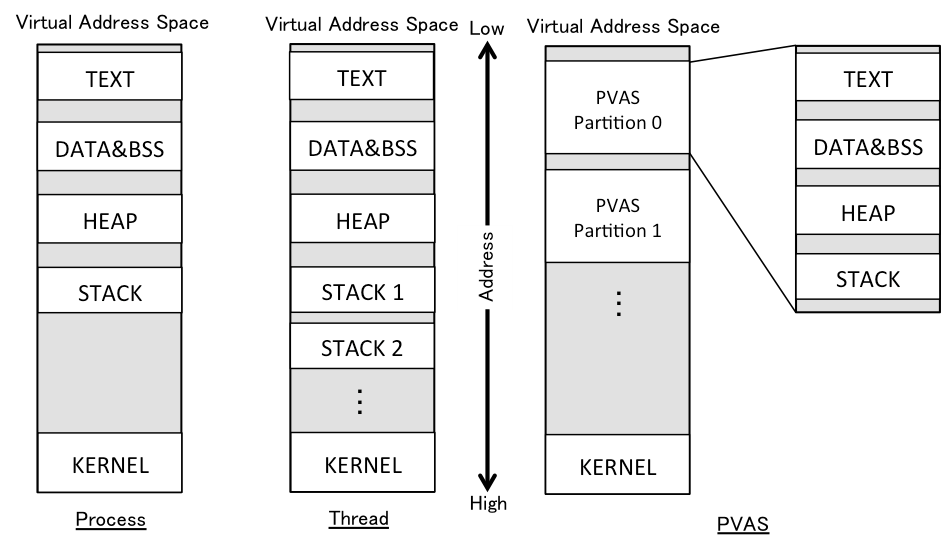
\includegraphics[width=0.7\textwidth, natwidth=678,natheight=391]{research/ishikawa/pvas.png}
\end{center}
 \caption{Partitioned Virtual Address Space}\locallabel{fig:pvas}
\end{figure}

It is already known that process oversubscription, which binds multiple parallel processes
to one CPU core, can hide the communication latency and reduce CPU
idle time. However, the lightweight OS kernels for Exascale systems
may no longer support OS task scheduling to reduce OS noise. Without
OS task scheduling, only one parallel process per CPU core is allowed
to run, and the process oversubscription is impossible. Even if the OS
task scheduling is supported, the overhead of the context switch
hinders the application performance and ruins the advantage of
process oversubscription. 

To tackle this issue, we proposed user-level process
(ULP) in FY2015. The user-level process is a process which can be scheduled in
the user-space. The ULP was implemented as an extension of PVAS. ULP
has the beneficial features of the user-level
thread. Meanwhile, it has its own program code and data like a
traditional process. By assigning a role of a parallel process to a
user-level process, high-performance process oversubscription can be
achieved without OS task scheduling. Moreover, the process
oversubscription utilizing ULP does not change the 
programming model of the parallel application.

The context switching times of conventional Linux process, Linux
thread and ULP over the number of execution entities are compared in
Figure \localref{fig:pvas-contextswitch}. Theoretically, there is no need
of calling any systemcall to switch user-level processes, however, the
privileged FS segment register is used to point Thread Local Storage
(TLS) must be switched at the time of context switch on the x86 CPU
architecture. As shown in Figure \localref{fig:pvas-contextswitch}, the
fastest one is ULP without switching the FS register, and send fastest
one is ULP with the FS switching. Anyway the context switching times
of conventional processes (KLP) and threads (KLP) are much higher than
those of ULPs.

\begin{figure}
\begin{center}
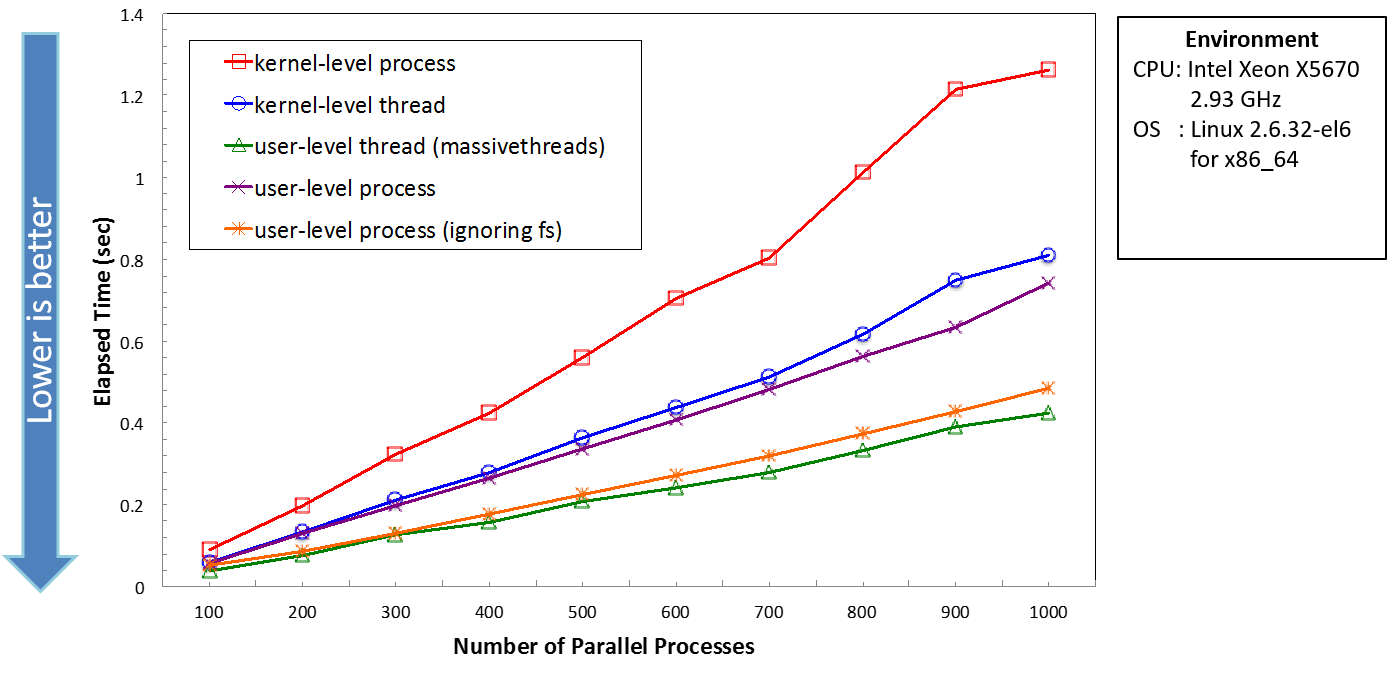
\includegraphics[width=0.8\textwidth,natwidth=1040,natheight=506] {research/ishikawa/pvas-contextswitch.png}
\end{center}
 \caption{Context Switching Time (KLP, KLT and ULP)}\locallabel{fig:pvas-contextswitch}
\end{figure}

%------------------------------------------------------------------------------
\subsection{Fault Resilience}
%------------------------------------------------------------------------------
With the increasing fault rate on high-end supercomputers, the topic
of fault tolerance has been gathering attention. To cope with this
situation, various fault-tolerance techniques are under investigation;
these include user-level, algorithm-based fault-tolerance techniques
and parallel execution environments that enable jobs to continue
following node failure. Even with these techniques, some programs,
such as stencil computation, having no dynamic load balancing function
may underperform after a failure recovery. Even when spare nodes are
present, they are not always substituted for failed nodes in an
effective way.

There are some questions of how spare nodes should be allocated, how
to substitute them for faulty nodes, and how much the communication
performance is affected by such a substitution. The third question
stems from the modification of the rank mapping by node substitutions,
which can incur additional message collisions. In a stencil
computation, rank mapping is done in a straightforward way on a
Cartesian network without incurring any message collisions. However,
once a substitution has occurred, the node-rank mapping may be
destroyed. Therefore, these questions must be answered in a way that
minimizes the degradation of communication performance.

\begin{figure}
\begin{center}
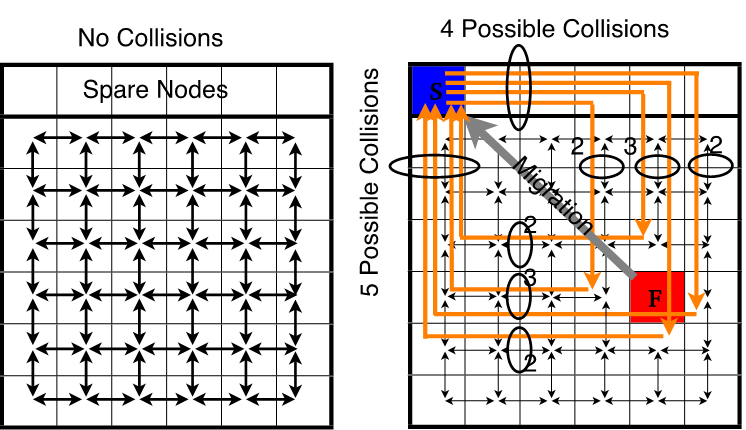
\includegraphics[width=0.7\textwidth,natwidth=373,natheight=215] {research/ishikawa/resilience1.png}
\end{center}
 \caption{Message collisions by substituting a failed node (5P-stencil)}\locallabel{fig:resilience1}
\end{figure}

Several spare-node allocation and node-substitution methods
had been proposed, compared and analyzed in terms of communication
performance(Figure \localref{fig:resilience1})\cite{hori2015}.

\begin{figure}
\begin{center}
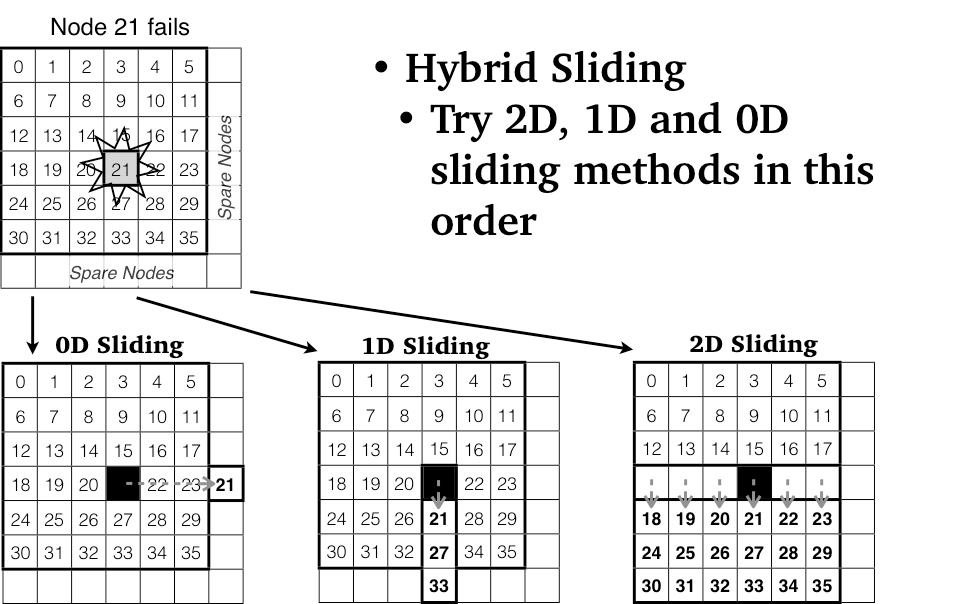
\includegraphics[width=0.7\textwidth,natwidth=958,natheight=604] {research/ishikawa/resilience2.png}
\end{center}
 \caption{Proposed Three Failed Node Substitution Methods}\locallabel{fig:resilience2}
\end{figure}

In FY2015, the proposed methods were evaluated using BlueGene Q (JUQUUEN at J\"ulich Supercomputing Center) and the K computer.
Figure \localref{fig:resilience2} shows the communication performance
degradation on the K computer\cite{yoshinaga2015}. The black lines represent the
simulation results with 3D mesh network having the same size with the
K computer evaluation (12x12x12) and the red lines represent the
evaluation results of the K computer. In all cases, the hybrid sliding
method is used. Left graph shows the cases with 7P stencil
communication pattern (4 MiB), upper right graph shows the cases with
the barrier collective communication, and the lower right graph shows
the allreduce collective communication (16 KiB). Figure
\localref{fig:resilience3} shows the communication performance on BG/Q with
the same way as in Figure cite{fig:resilience2}, unless otherwise
noted.

\begin{figure}
\begin{center}
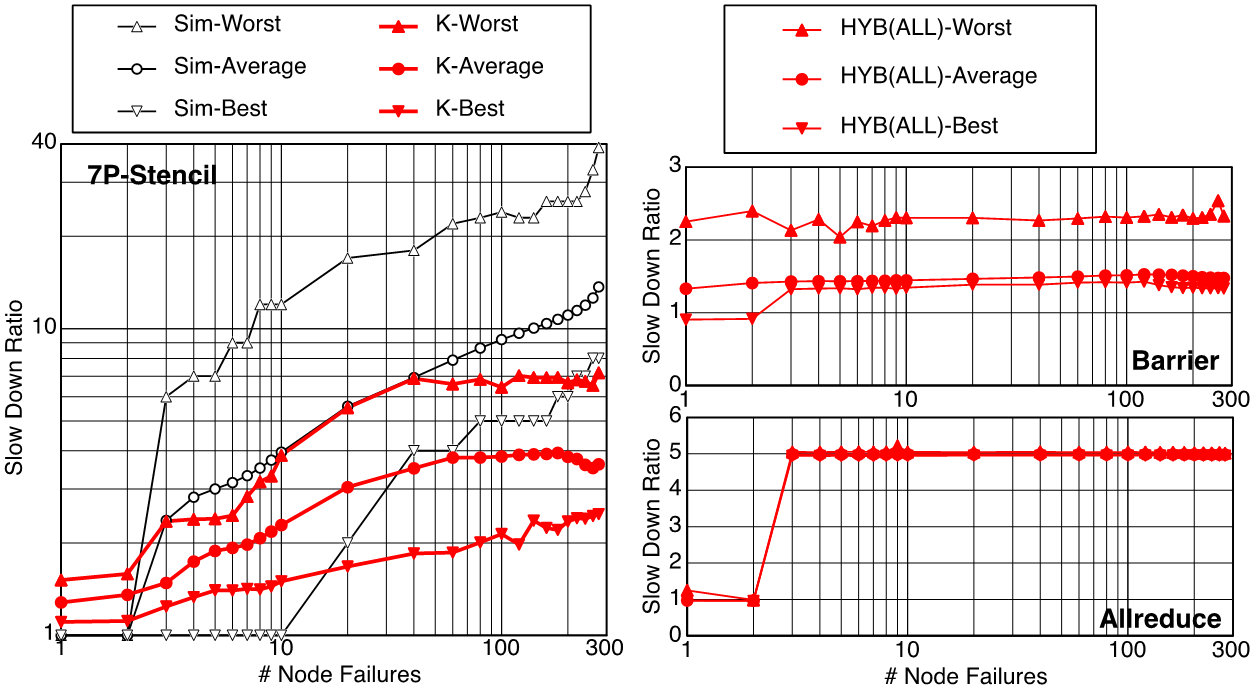
\includegraphics[width=0.8\textwidth,natwidth=628,natheight=347] {research/ishikawa/resilience3.png}
\end{center}
 \caption{Communication Performance Degradation by Using Spare Nodes 
the K computer (12x12x12)}\locallabel{fig:resilience3}
\end{figure}

\begin{figure}
\begin{center}
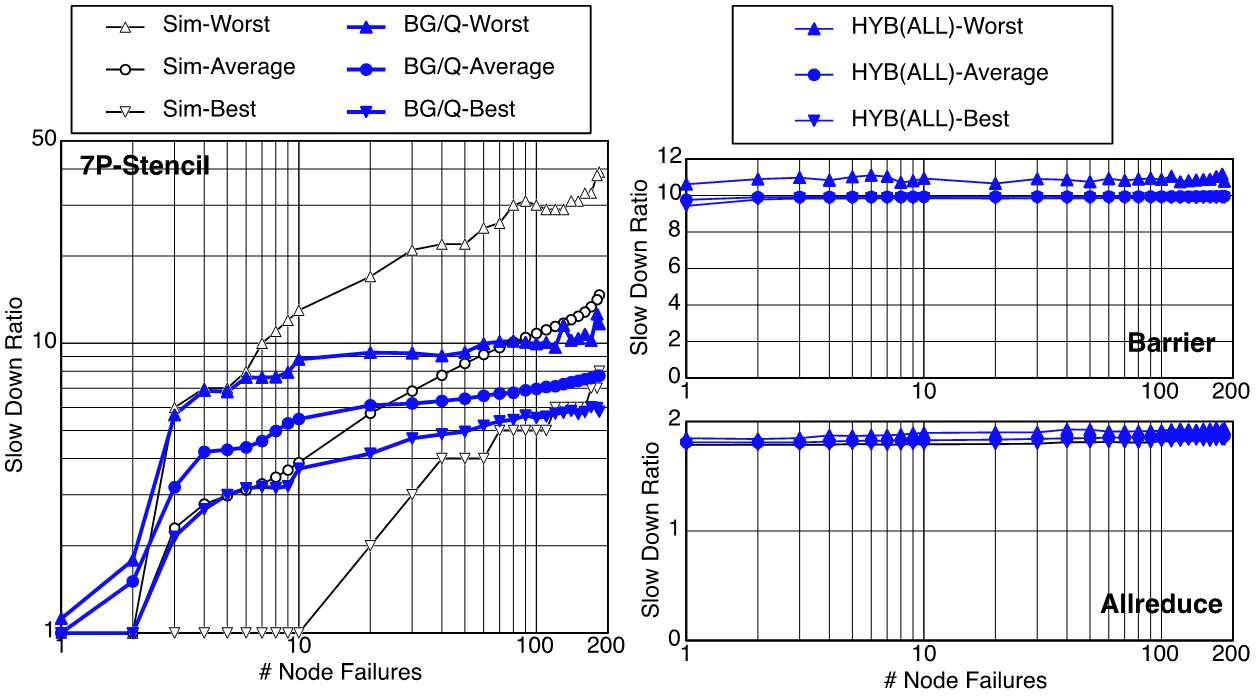
\includegraphics[width=0.8\textwidth,natwidth=904,natheight=499] {research/ishikawa/resilience4.png}
\end{center}
 \caption{Communication Performance Degradation by Using Spare Nodes 
the K computer (12x12x12)}\locallabel{fig:resilience4}
\end{figure}

As shown in Figures \localref{fig:resilience3} and
\localref{fig:resilience4}, the actual patterns of the stencil
communication performance degradation can vary in the K computer and
BG/Q. The collective communication performance degradation, however,
is relatively constant over the number of failed nodes.

%------------------------------------------------------------------------------
\subsection{Big data processing on the K computer}
%------------------------------------------------------------------------------
This research was conducted by collaboration between the Data
Acquisition team of RIKEN SPring-8 Center and the System Software
Research team of RIKEN AICS. The goal of this project is to establish
the path to discover the 3D structure of a molecule from a number of
XFEL (X-ray Free Electron Laser) snapshots. The K computer will be used to
analyze the huge data transmitted from RIKEN Harima where SACLA XFEL
facility is located.

In order to reduce quantum noise, each representative image must be
averaged out more than hundred images. In addition to this, the
sampled X-ray images must cover all possible orientations of the
molecule. The number of images, although it depends on desired
accuracy and the size of the molecule, can be one million in typical
cases. Thus, the massive power of the K computer is needed.

\begin{figure}
\begin{center}
 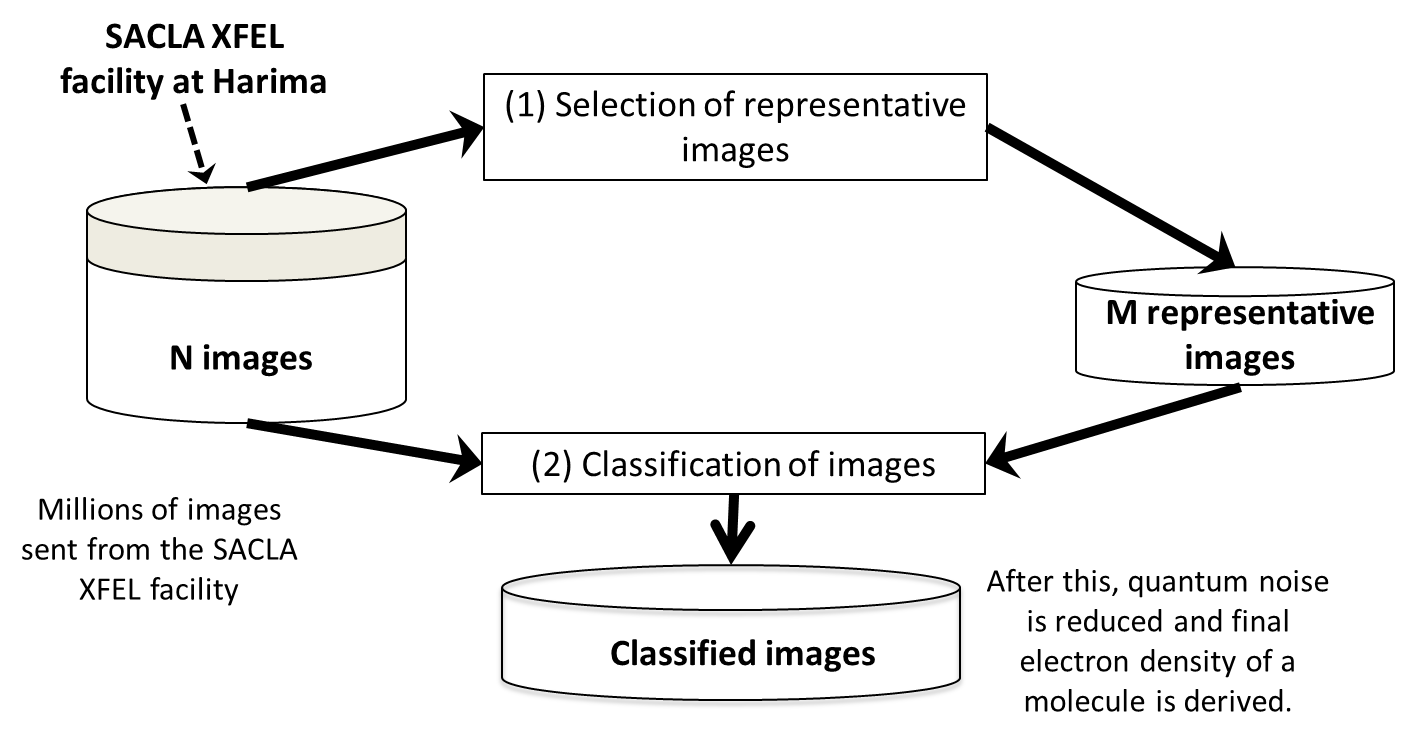
\includegraphics[width=0.7\textwidth,natwidth=1013,natheight=534] {research/ishikawa/carp1.png}
\end{center}
  \caption{Block diagram of the procedure running on the K computer}\locallabel{fig:carp1}
\end{figure}

We had developed a parallel software running on the K
computer to analyze images obtained by a light source, SACLA. The
developed software consists of two components as shown in \localref{fig:carp1}. The first phase is to select the representative images by a classic
clustering computation. Thus, all images must be compared with all
others. The second phase is to classify the rest of images into the
representative images. In this stage, we need to calculate for all
possible combinations of representative images and rest of the images.

\begin{figure}
\begin{center}
 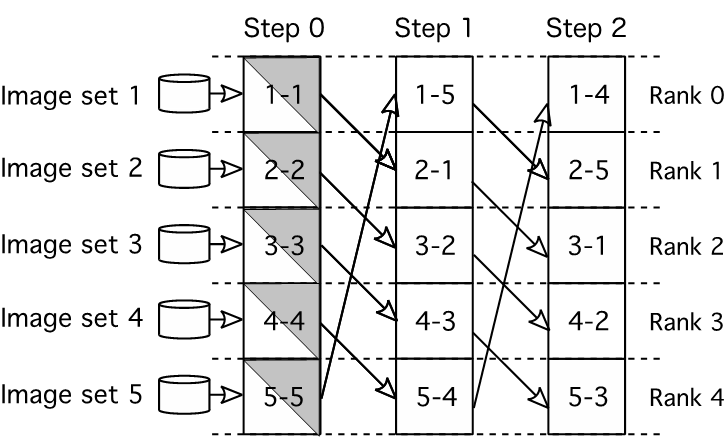
\includegraphics[width=0.7\textwidth,natwidth=523,natheight=316] {research/ishikawa/carp3.png}
\end{center}
  \caption{I/O minimization and load balancing}\locallabel{fig:carp3}
\end{figure}

After developing the first version of the program, 
we started to develop a new framework, named pCarp\cite{dist-carp}, to analyze any possible combination of two
records in a dataset processed by all participating processes. This
parallel processing can be used not only our target application (XFEL), but also can be
used to analyze gene sequencing data, images obtained by electron
microscopes, and so on. 
The pCarp framework takes care of parallelization and I/O minimization, while
sequential input program to read data from a file and sequential output
program to do the computation of two image data and to output the
result (Figure \localref{fig:carp3}). The most benefit of this framework is that 
the users do not need to write any
parallel programs, but write just two sequential programs; the input and output programs.

In FY2015, we found that the performance of the first version of pCarp was no good 
because there was a 
large overhead to transfer data between the pCarp framework and user sequential programs.
This overhead, however, was successfully reduced by introducing new data transfer mechanism.
New version of pCarp can not only on the K computer, but also on the conventional clusters.

%=============================================================================
\section{Schedule and Future Plan}
%=============================================================================
Results of the System Software Research Team are being taken over by the
System Software Development Team of Flagship 2020 project.
The members mainly will work for the Flagship 2020 project from the
next year.  The MPI-IO library with the EARTH optimization will be
available at the K computer in the next year.  The team will mainly
maintain the published software.

\long\def\mycomment#1{}
\mycomment{
\begin{itemize}
\item
The PRDMA will also be applied to a prototype implementation of MPI-4 Persistent Collectives in our MPICH on K computer.

\item
OFI/LLC V1.2 for Intel Omni-path architecture and RMPI V1.2 based on
MPICH-3.2 will be developed in FY2016.
%The development will focus on development of the missing MPI functions
%(i.e. connect/accept) and adapting to Intel Omni-path
%architecture. OFI/LLC V1.3 for Intel Omni-path architecture and RMPI
%V1.3 based on MPICH-3.3 will be developed until the end of March. The
%development will focus on bringing optimizations in OFI/LLC to the
%master branch of the source code repository of OFI and trying to
%integrate the interface extensions for inter-domain communications
%into the OFI standard.

\item
The EARTH optimization will be available at the K computer after minor
modifications. Further optimization such as tuning scheme for the
number of I/O requests in throttling will be considered.

\item New Process / Thread Model\\
Integration of the proposed task model with the McKernel which is under
development by AICS System Software Development team is planned.
% Also,
%we are doing a collaborative research with ANL on the User-level
%process which was developed in last FY2013 to enhance the performance
%of irregular applications.
%
%\item Fault Resilience\\
%Based on the investigation in FY2014, we will start developing a
%framework to allow user applications to be fault-resilient easily.
\end{itemize}
}


%%% DO NOT EDIT BELOW

\section{Publications}

%\printbibliography[keyword=journal, heading=subbibliography, title={Journal Articles}, prefixnumbers={1-}, resetnumbers=true]
%\printbibliography[keyword=proceedings, heading=subbibliography, title={Conference Papers}, prefixnumbers={2-}, resetnumbers=true]
%\printbibliography[keyword=invited, heading=subbibliography, title={Invited Talks}, prefixnumbers={3-}, resetnumbers=true]
%\printbibliography[keyword=poster, heading=subbibliography, title={Posters and Presentations}, prefixnumbers={4-}, resetnumbers=true]
%\printbibliography[keyword=deliverable, heading=subbibliography, title={Patents and Deliverables}, prefixnumbers={5-}, resetnumbers=true]

\printbibliography[keyword=journal, heading=subbibliography, title={Journal Articles}, resetnumbers=true]
\printbibliography[keyword=proceedings, heading=subbibliography, title={Conference Papers}]
\printbibliography[keyword=invited, heading=subbibliography, title={Invited Talks}]
\printbibliography[keyword=poster, heading=subbibliography, title={Posters and Presentations}]
\printbibliography[keyword=deliverable, heading=subbibliography, title={Patents and Deliverables}]

\end{refsection}

